\documentclass[11pt]{article}
\usepackage[margin=1in]{geometry}
\usepackage{amsmath,amssymb}
\usepackage{graphicx}
\usepackage{hyperref}
\usepackage{booktabs}
\usepackage{natbib}
\hypersetup{colorlinks=true,linkcolor=blue,citecolor=blue,urlcolor=blue}

\title{Orch-OR Visualizer: An Interactive, Calibrated Toy Model of\\Orchestrated Objective Reduction for Teaching and Critique}
\author{John Seong\\ \small Chief Scientific Officer, Orchestr Aerospace Inc.\\ \small \href{mailto:wonmor@yahoo.com}{wonmor@yahoo.com}}
\date{October 2026}

\begin{document}
\maketitle

\begin{abstract}
Orchestrated Objective Reduction (Orch-OR) is the Penrose--Hameroff proposal that conscious moments are gravitationally induced collapses of quantum superpositions in neuronal microtubules. The theory is unusual among theories of consciousness in making specific numerical claims: a collapse time $\tau \approx \hbar/E_G$, a calibration of roughly $2\times10^{10}$ tubulins per 25~ms ``moment'', and a direct conflict with decoherence estimates spanning nine orders of magnitude. We present \emph{Orch-OR Visualizer}, an open-source interactive model for iOS and the web that renders a 13-protofilament microtubule lattice in which tubulin superposition seeds, spreads by ``orchestration'', accumulates gravitational self-energy, and undergoes objective reduction when $\int E_G\,dt$ reaches $\hbar$. The model is calibrated to Hameroff and Penrose (2014), exposes every quantity on screen, and includes a decoherence switch set to the Tegmark (2000) and Hagan--Hameroff--Tuszynski (2002) estimates so that the central empirical dispute can be experienced rather than read about. We describe the model, its deliberate simplifications, a companion calculator, and the design choices made to present a contested theory without endorsing it. The software is intended as a teaching instrument and a shared reference implementation of the theory's arithmetic, not as evidence for or against Orch-OR.
\end{abstract}

\section{Introduction}
Orch-OR \citep{penrose1989,penrose1994,hameroff1996,hameroff2014} proposes that consciousness arises from quantum computation in the microtubules of neurons, terminated by a gravitational self-collapse that Penrose calls objective reduction (OR). The proposal has been widely criticised, most influentially on decoherence grounds \citep{tegmark2000,koch2006}, and defended \citep{hagan2002}; recent experimental work on anaesthetic action at microtubules \citep{khan2024} and on collective optical effects in tubulin \citep{babcock2024,kalra2023} is cited by proponents as supportive, while direct tests of gravity-related collapse have constrained the simplest Di\'osi--Penrose variants \citep{donadi2021}.

Whatever its standing, Orch-OR has a property that makes it unusually teachable: its claims are quantitative. Students and critics alike can ask how many tubulins, how long a coherence time, and how many neurons the theory requires, and compare those numbers with independent estimates. In practice these numbers are scattered across papers and rarely computed by readers. We built a small interactive model that puts them on one screen and lets the user move the dials.

\paragraph{Contribution.} (i) A real-time toy model of orchestrated superposition growth and objective reduction on a geometrically faithful microtubule lattice, with the collapse criterion $\int E_G\,dt \ge \hbar$ and the Hameroff--Penrose calibration; (ii) a decoherence mode that reproduces, qualitatively, the Tegmark and Hagan et al.\ regimes; (iii) a Di\'osi--Penrose calculator that places all the relevant timescales on one logarithmic axis; (iv) an open-source implementation for iOS (Swift, SceneKit) and the web (three.js), with a didactic layer that presents both the theory and its criticisms with references. We claim no new physics.

\section{Background}
\subsection{Objective reduction}
Penrose's criterion \citep{penrose1996}, reached independently by Di\'osi \citep{diosi1989}, is that a superposition of two mass distributions is unstable on a timescale
\begin{equation}
\tau \;\approx\; \frac{\hbar}{E_G},
\label{eq:tau}
\end{equation}
where $E_G$ is the gravitational self-energy of the difference between the two distributions. For a tubulin dimer displaced by roughly the diameter of an atomic nucleus, Hameroff and Penrose \citep{hameroff2014} estimate that about $2\times10^{10}$ tubulins in coherent superposition give $\tau \approx 25$~ms, which they identify with the period of 40~Hz gamma synchrony. With $\sim10^9$ tubulins per neuron and $0.1\%$ participation, this corresponds to on the order of $2\times10^4$ neurons.

\subsection{Orchestration}
``Orchestration'' refers to microtubule-associated proteins, synaptic input and cellular biochemistry shaping which superpositions form and when they reduce, so that reductions are structured rather than random. In the model, orchestration is represented by a single coupling parameter governing how readily a dimer in superposition recruits its lattice neighbours.

\subsection{The decoherence objection}
Tegmark \citep{tegmark2000} estimated decoherence times for microtubule superpositions of order $10^{-13}$~s. Hagan, Hameroff and Tuszynski \citep{hagan2002} argued that the relevant system was mis-modelled and obtained $10^{-5}$--$10^{-4}$~s with screening by ordered water and counter-ions. Both figures are far below 25~ms; the disagreement is about how far.

\section{The model}
\subsection{Lattice}
The lattice has $P=13$ protofilaments and $R=30$ rings, i.e.\ $N=390$ dimers, arranged on a cylinder of unit radius with axial spacing $\Delta z$ and a 3-start helical offset of $3\Delta z/P$ per protofilament, matching the B-lattice geometry of real microtubules. Each dimer has a state $s_i \in \{A, B, \mathrm{S}\}$: two classical conformations and a superposed state.

\subsection{Representation scale}
A 390-dimer lattice cannot reach $2\times10^{10}$ tubulins, so each displayed dimer stands for $10^{x}$ real dimers distributed across many neurons, with $x$ a user control (default $x=7.7$, so a fully superposed lattice represents $1.95\times10^{10}$ tubulins). The effective number in superposition is $N_\mathrm{eff} = 10^{x}\,|\{i : s_i = \mathrm{S}\}|$.

\subsection{Dynamics}
Simulated time advances at $1/k$ of wall-clock time (default $k=40$). Per step of simulated duration $dt$:
\begin{enumerate}
\item \textbf{Seeding.} With probability $0.03\,dt_\mathrm{ms}$ a random dimer enters S.
\item \textbf{Orchestration.} Each dimer in S recruits each of its four lattice neighbours into S with probability $\min(1, 0.5\,\gamma\, dt_\mathrm{ms})$, where $\gamma\in[0,1]$ is the orchestration control.
\item \textbf{Decoherence (optional).} Each dimer in S reverts to a random classical state with probability $\min(1, dt/t_\mathrm{dec})$, where $t_\mathrm{dec}$ is a user control with presets $10^{-13}$~s and $10^{-4}$~s.
\item \textbf{Self-energy and action.} $E_G = N_\mathrm{eff}\,\epsilon$ with $\epsilon = \hbar/(0.025\,\mathrm{s}\times 2\times10^{10}) \approx 2.1\times10^{-43}$~J per tubulin, and the accumulated action $S \leftarrow S + E_G\,dt$ (reset to zero whenever no dimer is superposed).
\item \textbf{Objective reduction.} When $S \ge \hbar$, every dimer in S is assigned a classical state, an event is logged with $(t, N_\mathrm{eff}, \tau)$, and $S\leftarrow 0$.
\end{enumerate}
The criterion $\int E_G\,dt \ge \hbar$ reduces to $\tau = \hbar/E_G$ for constant $E_G$ (Eq.~\ref{eq:tau}) and extends it naturally to a growing superposition, which is the situation the theory describes. The outcome of each reduction is drawn at random; Orch-OR holds it to be non-computable, which a simulation cannot represent, and the interface says so.

\subsection{Readouts}
The interface shows, continuously: the number of superposed dimers and $N_\mathrm{eff}$; $E_G$; $\tau = \hbar/E_G$ for the current superposition; the fraction $S/\hbar$; the number of OR events; and the recent event rate in Hz, which the user can compare with the 40~Hz target. A timeline tab plots $|\{i: s_i=\mathrm{S}\}|(t)$ with event markers.

\begin{figure}[t]
\centering
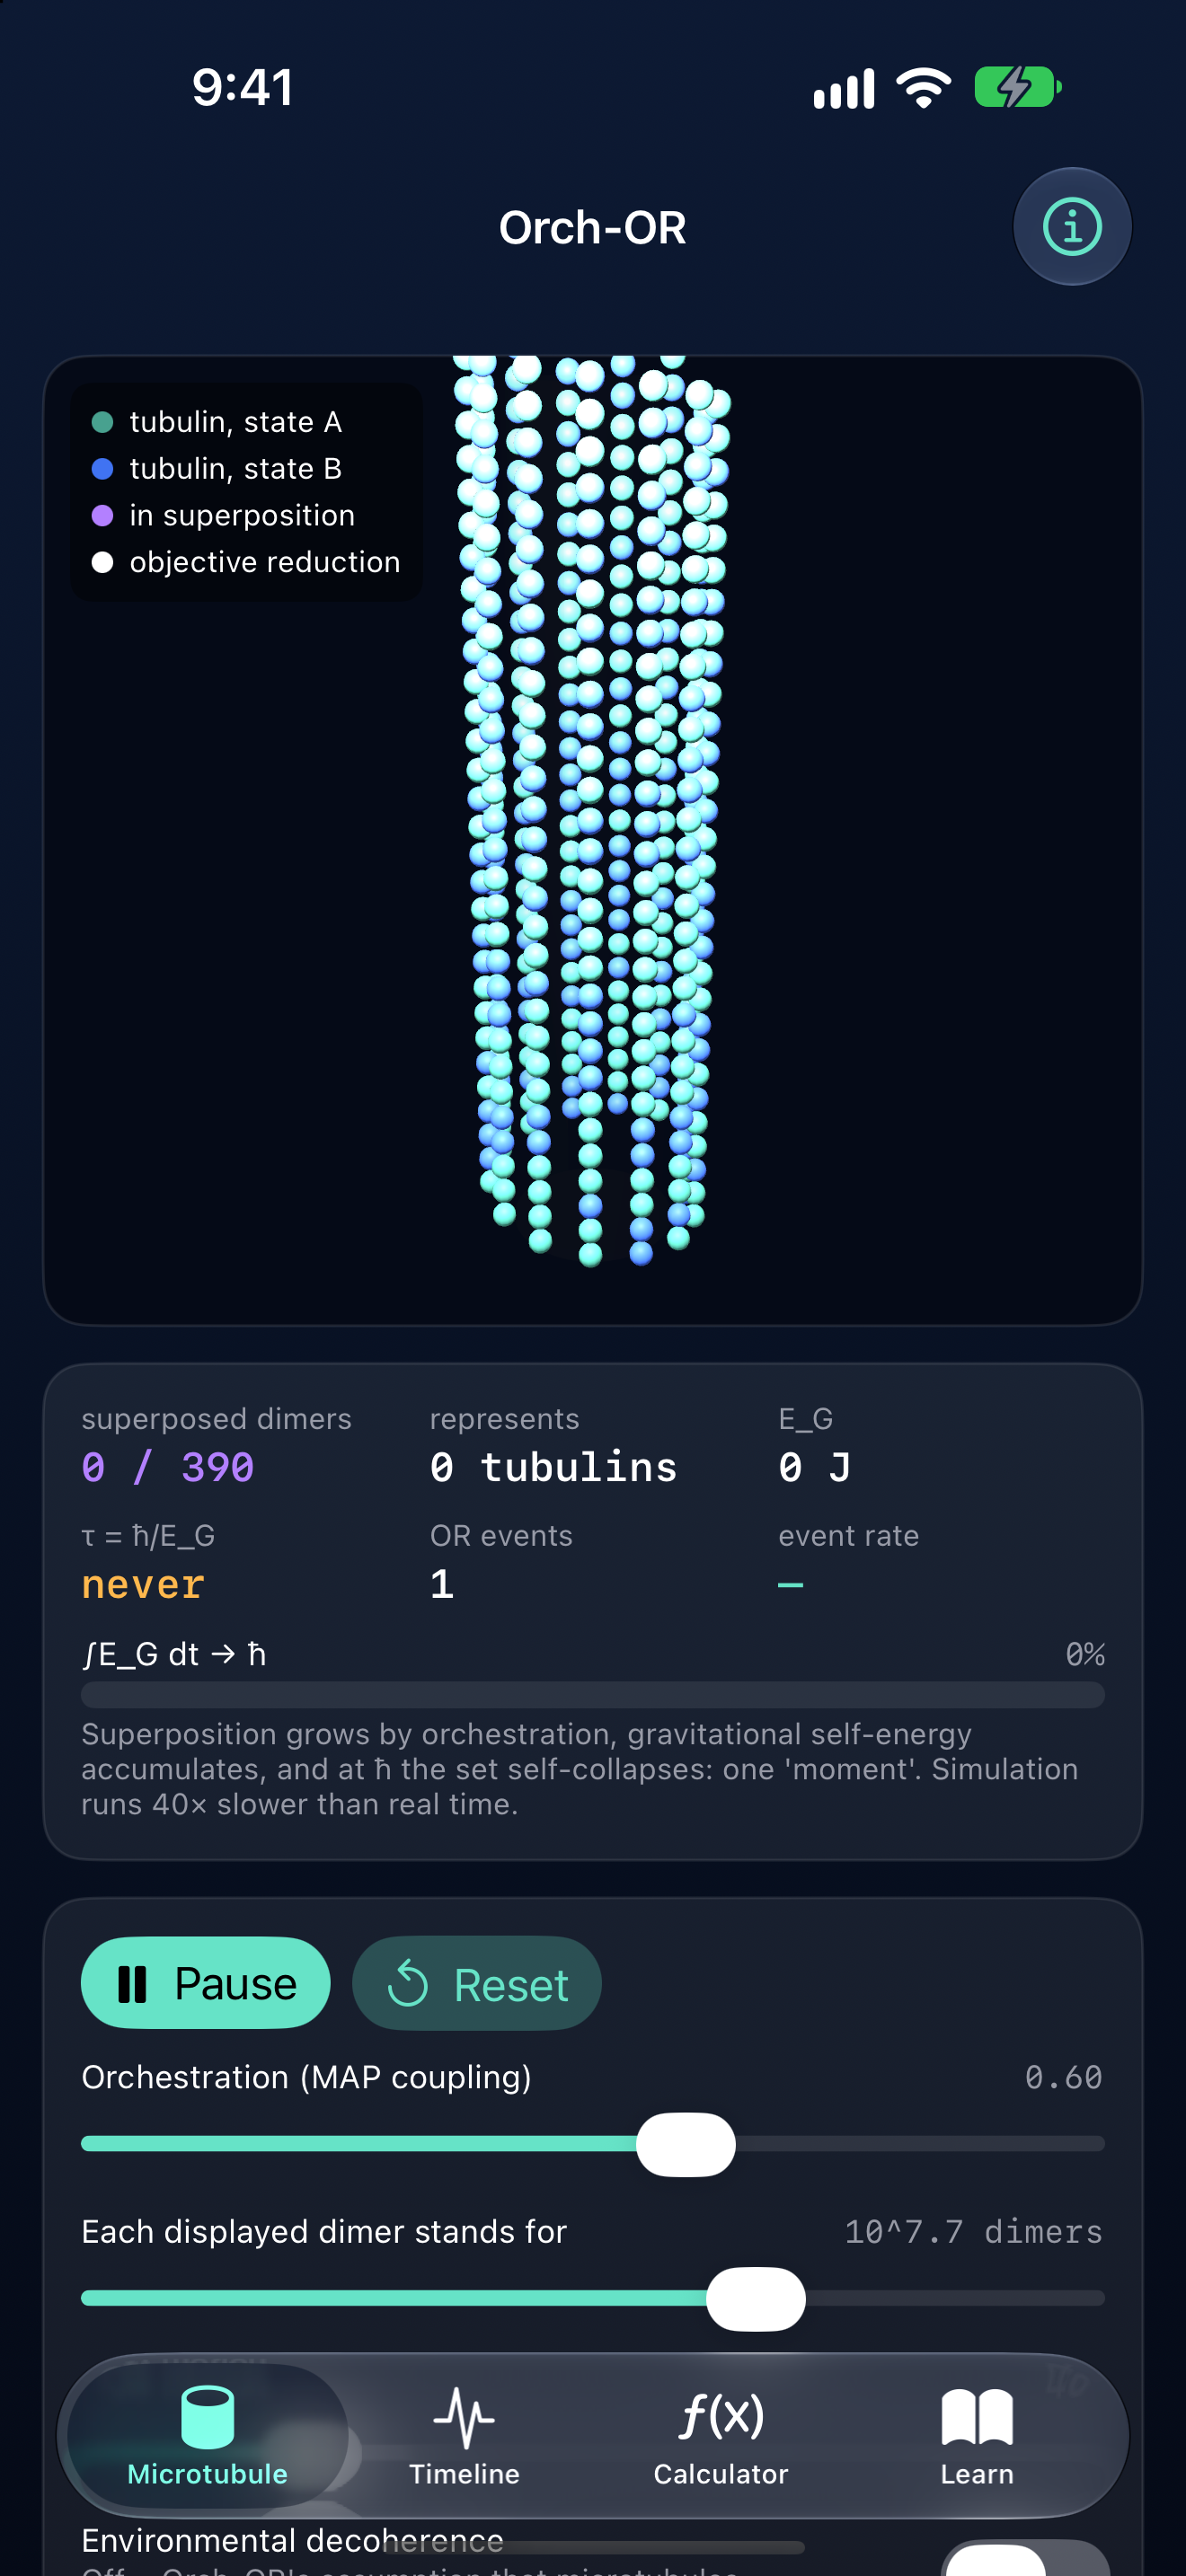
\includegraphics[width=0.36\textwidth]{fig-lattice.png}\hfill
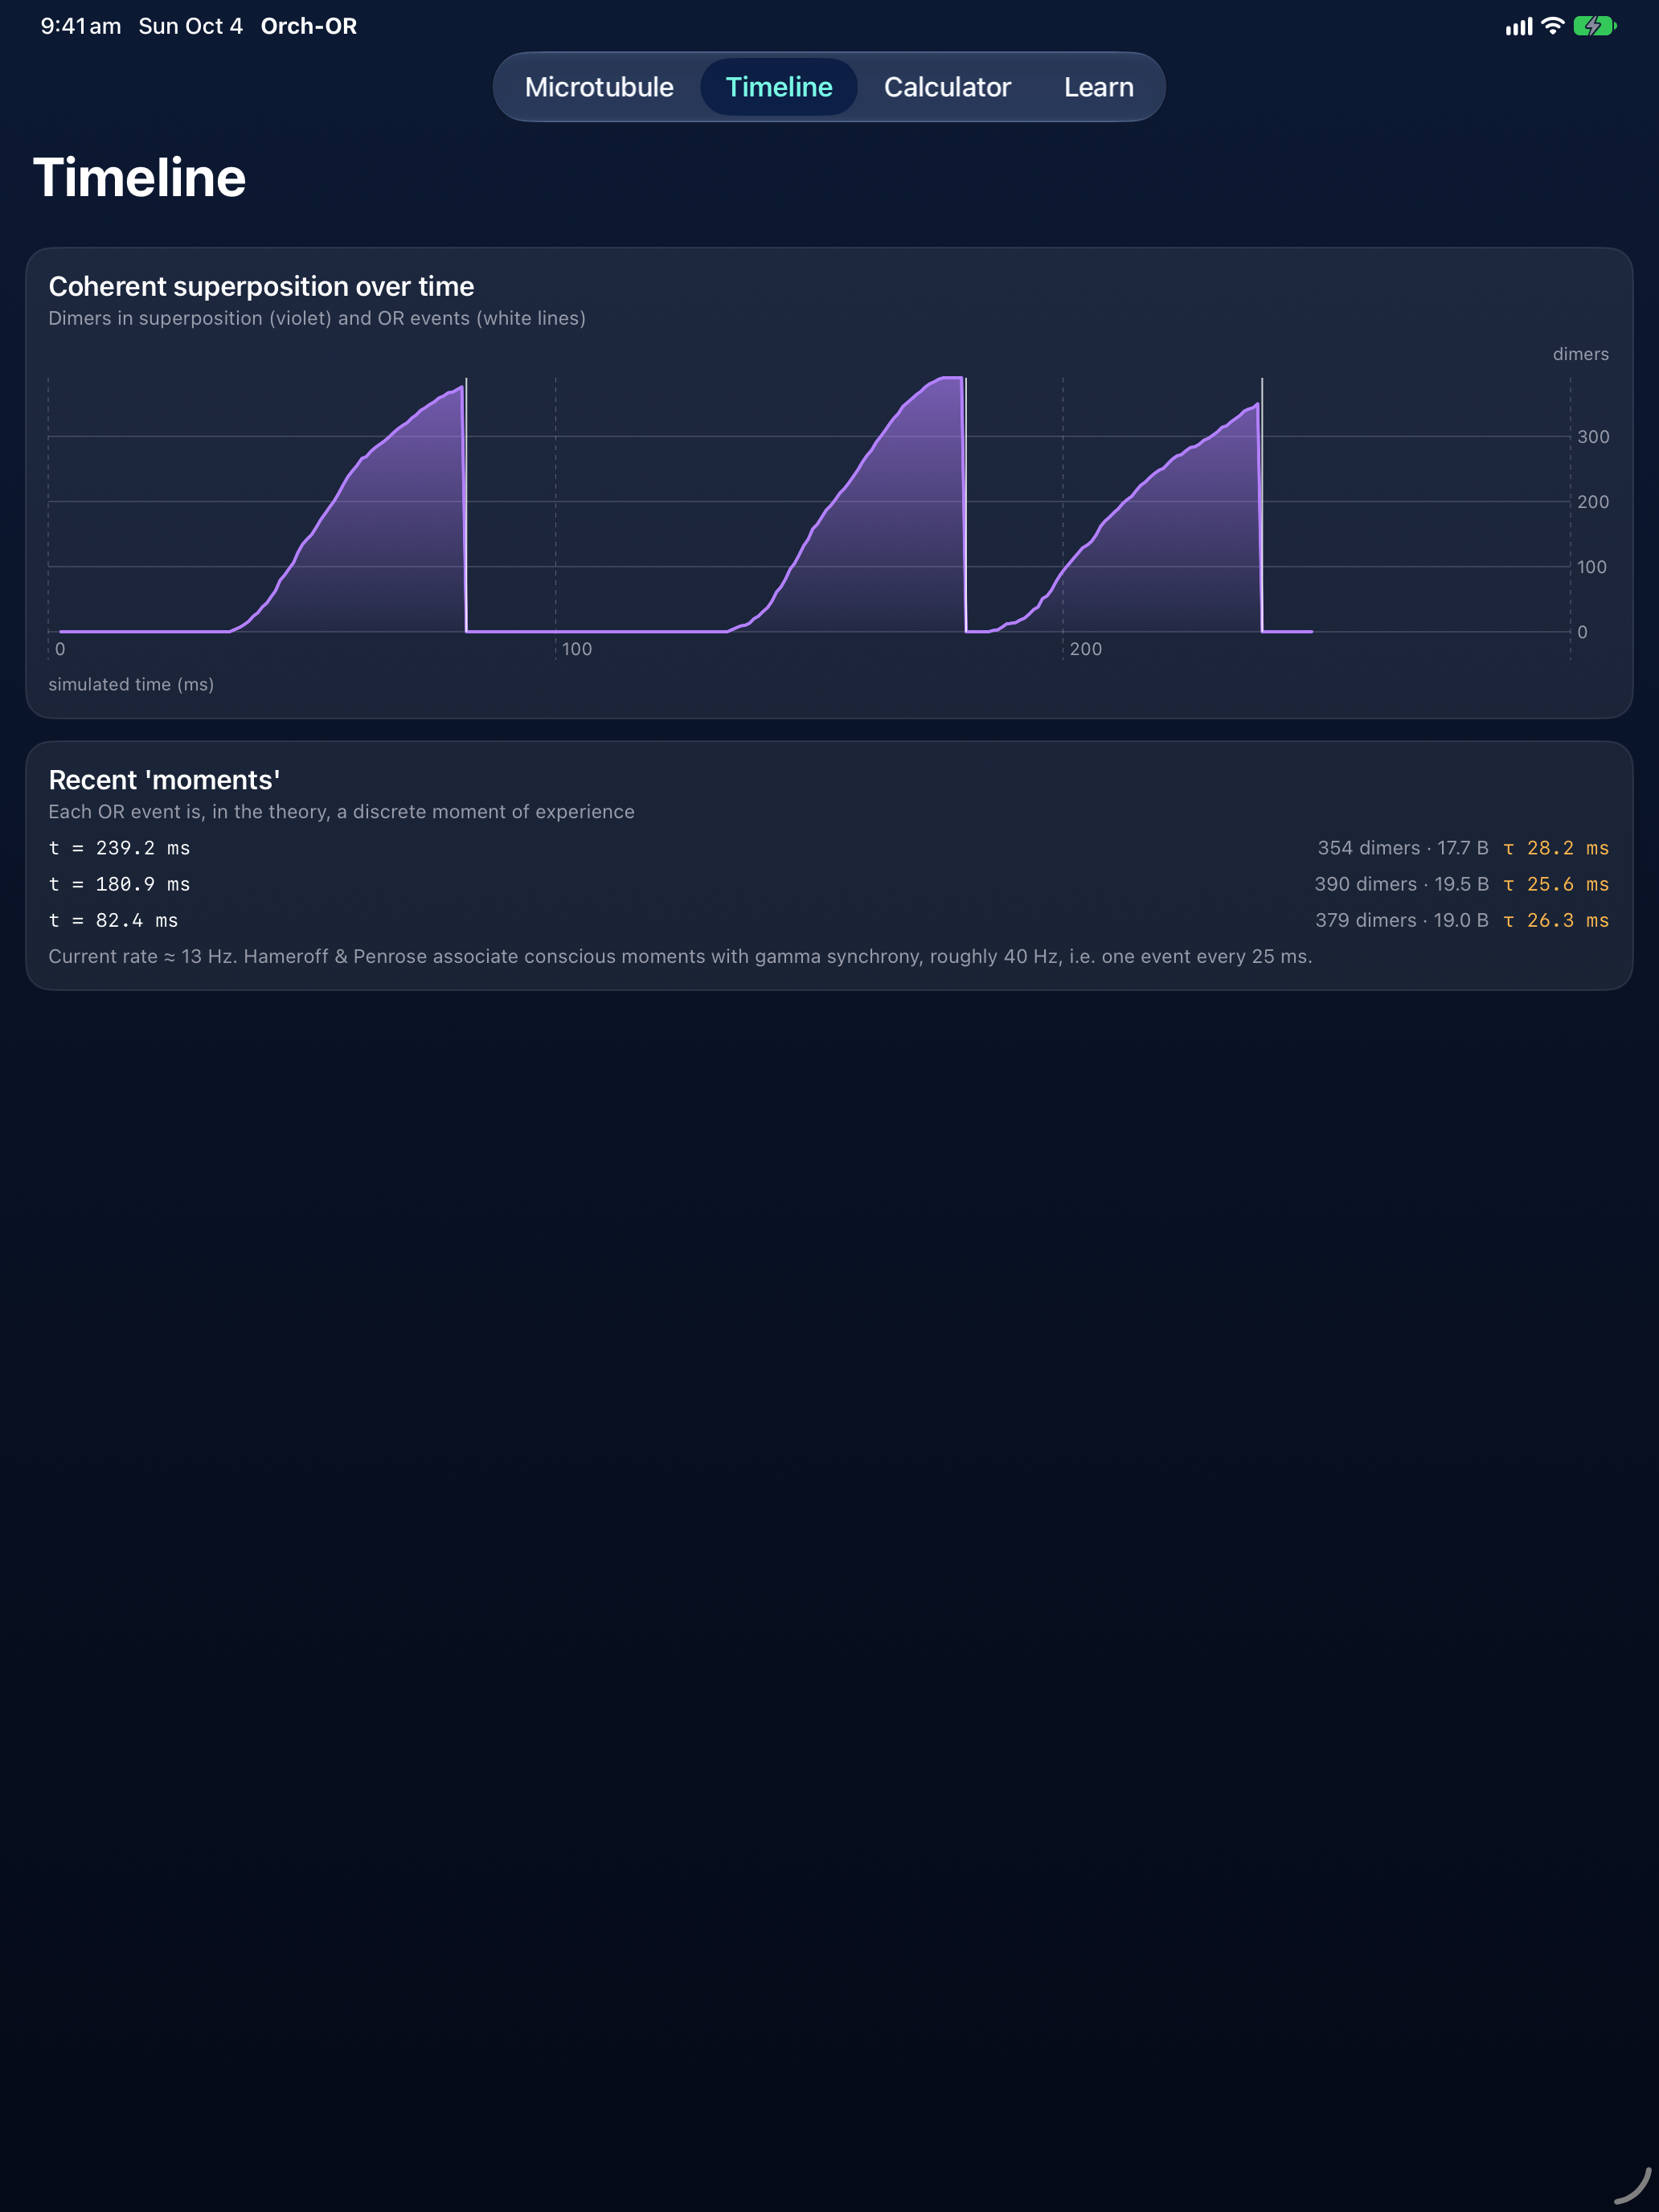
\includegraphics[width=0.60\textwidth]{fig-timeline.png}
\caption{Left: the microtubule lattice and live readouts on iPhone. Right: coherence over simulated time with objective-reduction events (white lines) on iPad; at the default calibration the model settles near 25--28~ms per event.}
\end{figure}

\subsection{Calculator}
A separate calculator evaluates Eq.~\ref{eq:tau} for $N$ from $10^6$ to $10^{13}$ tubulins and the implied neuron count for a chosen participation fraction, and plots the resulting $\tau$ against 25~ms, 500~ms, and the two decoherence estimates on a single logarithmic axis.

\section{What the model shows}
At the default calibration the lattice produces events at intervals of roughly 25--30~ms of simulated time, as it must: the parameters were chosen to reproduce the Hameroff--Penrose figure. The value of the model is in what happens when the user departs from that point. Lowering orchestration lengthens intervals and produces smaller, more frequent partial collapses; lowering the representation scale pushes $\tau$ to seconds. Enabling decoherence at the Hagan et al.\ value prevents coherence from ever exceeding a handful of dimers; at the Tegmark value, superposition is extinguished within a frame. The user sees directly that the theory's viability hinges on $t_\mathrm{dec} \gtrsim \tau$, and how large the gap is under each estimate.

\section{Limitations}
This is a teaching model. The recruitment and seeding rates, the choice of four lattice neighbours, the random post-collapse states and the representation scale are illustrative, not derived. No quantum state is simulated; ``superposition'' is a label on a classical cellular automaton. $E_G$ is linear in the number of tubulins, which follows the Hameroff--Penrose estimate but ignores spatial structure. The model does not address how a reduction would influence neuronal firing, nor the non-computability claim. It should not be read as evidence for or against Orch-OR, and the software states this on its About screen.

\section{Design for a contested theory}
The didactic layer presents nine short sections: the claim, microtubules, tubulin as a qubit, objective reduction, orchestration, the 40~Hz argument, the decoherence objection, the evidence proponents cite, and the theory's current standing. Criticisms are given the same prominence as claims, with primary references. In our view this is the right posture for software about a minority scientific position: make the arithmetic reproducible, show both sides, and let the numbers argue.

\section{Availability}
Orch-OR Visualizer is available for iPhone and iPad on the App Store and as a browser version at \url{https://wonmor.github.io/orch-or/}. Source code (Swift/SceneKit for iOS, three.js for the web) is released under the MIT licence at \url{https://github.com/wonmor/OrchOR} and \url{https://github.com/wonmor/orch-or}. A companion app by the same author, \emph{Orch Neural Network} (\url{https://github.com/wonmor/OrchNeuralNetwork}), applies the same approach to a classical system, running a small transformer language model on device and exposing its attention, activations and weights.

\section*{Acknowledgements and disclosure}
The software and this manuscript were produced with substantial AI assistance (Claude, Anthropic) under the author's direction. The author is responsible for the design, the framing, the choice of calibration and references, and all claims made here.

\bibliographystyle{plainnat}
\begin{thebibliography}{99}
\bibitem[Babcock et al.(2024)]{babcock2024} N.~S. Babcock, G.~Montes-Cabrera, K.~E. Oberhofer, M.~Chergui, G.~L. Celardo, P.~Kurian. Ultraviolet superradiance from mega-networks of tryptophan in biological architectures. \emph{J. Phys. Chem. B} 128 (2024).
\bibitem[Di\'osi(1989)]{diosi1989} L.~Di\'osi. Models for universal reduction of macroscopic quantum fluctuations. \emph{Phys. Rev. A} 40, 1165 (1989).
\bibitem[Donadi et al.(2021)]{donadi2021} S.~Donadi, K.~Piscicchia, C.~Curceanu, L.~Di\'osi, M.~Laubenstein, A.~Bassi. Underground test of gravity-related wave function collapse. \emph{Nature Physics} 17, 74 (2021).
\bibitem[Hagan et al.(2002)]{hagan2002} S.~Hagan, S.~R. Hameroff, J.~A. Tuszy\'nski. Quantum computation in brain microtubules: Decoherence and biological feasibility. \emph{Phys. Rev. E} 65, 061901 (2002).
\bibitem[Hameroff and Penrose(1996)]{hameroff1996} S.~Hameroff, R.~Penrose. Orchestrated reduction of quantum coherence in brain microtubules: A model for consciousness. \emph{Mathematics and Computers in Simulation} 40, 453 (1996).
\bibitem[Hameroff and Penrose(2014)]{hameroff2014} S.~Hameroff, R.~Penrose. Consciousness in the universe: A review of the `Orch OR' theory. \emph{Physics of Life Reviews} 11, 39 (2014).
\bibitem[Kalra et al.(2023)]{kalra2023} A.~P. Kalra et al. Electronic energy migration in microtubules. \emph{ACS Central Science} 9, 352 (2023).
\bibitem[Khan et al.(2024)]{khan2024} S.~Khan, Y.~Huang, D.~Timu\c{c}in, S.~Bailey, S.~Lee, J.~Lopes, E.~Gaunce, J.~Mosberger, M.~Zhan, B.~Abdelrahman, X.~Zeng, M.~C. Wiest. Microtubule-stabilizer epothilone B delays anesthetic-induced unconsciousness in rats. \emph{eNeuro} 11(8) (2024).
\bibitem[Koch and Hepp(2006)]{koch2006} C.~Koch, K.~Hepp. Quantum mechanics in the brain. \emph{Nature} 440, 611 (2006).
\bibitem[Penrose(1989)]{penrose1989} R.~Penrose. \emph{The Emperor's New Mind}. Oxford University Press (1989).
\bibitem[Penrose(1994)]{penrose1994} R.~Penrose. \emph{Shadows of the Mind}. Oxford University Press (1994).
\bibitem[Penrose(1996)]{penrose1996} R.~Penrose. On gravity's role in quantum state reduction. \emph{General Relativity and Gravitation} 28, 581 (1996).
\bibitem[Tegmark(2000)]{tegmark2000} M.~Tegmark. Importance of quantum decoherence in brain processes. \emph{Phys. Rev. E} 61, 4194 (2000).
\end{thebibliography}
\end{document}
